\documentclass[12pt,a4paper]{article}
\usepackage{amsmath,amssymb,amsfonts}
\usepackage{graphicx}
\usepackage{hyperref}
\usepackage{geometry}
\usepackage{float}
\usepackage{caption}
\usepackage{subcaption}
\usepackage{enumitem}
\usepackage{xcolor}
\usepackage{fancyhdr}
\usepackage{titlesec}
\usepackage{booktabs}
\usepackage{array}
\usepackage{multirow}

\geometry{left=2.5cm,right=2.5cm,top=2.5cm,bottom=2.5cm}

\definecolor{primary}{RGB}{41,128,185}
\definecolor{secondary}{RGB}{231,76,60}
\definecolor{accent}{RGB}{46,204,113}

\hypersetup{
    colorlinks=true,
    linkcolor=primary,
    urlcolor=primary,
    citecolor=primary
}

\titleformat{\section}
{\normalfont\Large\bfseries\color{primary}}
{\thesection}{1em}{}

\titleformat{\subsection}
{\normalfont\large\bfseries\color{primary!80}}
{\thesubsection}{1em}{}

\pagestyle{fancy}
\fancyhf{}
\fancyhead[L]{\textcolor{primary}{Mathematical Software - Project}}
\fancyhead[R]{\thepage}
\renewcommand{\headrulewidth}{0.5pt}
\renewcommand{\headrule}{\hbox to\headwidth{\color{primary}\leaders\hrule height \headrulewidth\hfill}}

\graphicspath{{./}}

\title{
    \vspace{1cm}
    {\Huge \textbf{Numerical Methods Project}} \\
    \vspace{0.5cm}
    {\Large Interpolation, Data Analysis, and Numerical Integration} \\
    \vspace{1.5cm}
}
\author{
    \textbf{Name:} Arad Shafiee \\
    \textbf{Student ID:} 40312029 \\
    \textbf{Course:} Mathematical Software \\
    \textbf{Date:} July 2025 (Tir 1405)
}
\date{}

\begin{document}

\maketitle
\thispagestyle{empty}
\newpage

\tableofcontents
\newpage

\listoffigures
\newpage

\listoftables
\newpage

\section{Project 1: Interpolation Methods}

\subsection{Introduction}
This section implements two interpolation methods: Lagrange Interpolation and Cubic Spline Interpolation. These methods approximate functions passing through given discrete data points.

\subsection{Data Points}
The given data points are shown in Table 1.

\begin{table}[H]
\centering
\caption{Given Data Points}
\label{tab:data_points}
\begin{tabular}{|c|c|c|c|c|c|c|}
\hline
$x$ & 1 & 2 & 3 & 4 & 5 & 6 \\
\hline
$y$ & 1 & 3 & 5 & 8 & 5 & 2 \\
\hline
\end{tabular}
\end{table}

\subsection{Lagrange Interpolation}
The Lagrange interpolation polynomial is defined as:
\[
P(x) = \sum_{i=0}^{n} y_i L_i(x)
\]
where the Lagrange basis polynomials are given by:
\[
L_i(x) = \prod_{\substack{j=0 \\ j \neq i}}^{n} \frac{x - x_j}{x_i - x_j}
\]

The resulting polynomial of degree 5 is:
\[
P(x) = -0.7083x^5 + 9.8333x^4 - 50.8333x^3 + 121.1667x^2 - 131.4583x + 53
\]

\subsection{Cubic Spline Interpolation}
The natural cubic spline uses piecewise cubic polynomials defined on each interval:
\[
S_i(x) = a_i(x-x_i)^3 + b_i(x-x_i)^2 + c_i(x-x_i) + d_i, \quad x \in [x_i, x_{i+1}]
\]

The coefficients for each interval are shown in Table 2.

\begin{table}[H]
\centering
\caption{Cubic Spline Coefficients}
\label{tab:spline_coeffs}
\begin{tabular}{|c|c|c|c|c|}
\hline
\textbf{Interval} & \textbf{$a_i$} & \textbf{$b_i$} & \textbf{$c_i$} & \textbf{$d_i$} \\
\hline
$[1,2]$ & 1.0000 & 2.1866 & 0.0000 & -0.1866 \\
$[2,3]$ & 3.0000 & 1.6268 & -0.5598 & 0.9330 \\
$[3,4]$ & 5.0000 & 3.3062 & 2.2392 & -2.5455 \\
$[4,5]$ & 8.0000 & 0.1483 & -5.3971 & 2.2488 \\
$[5,6]$ & 5.0000 & -3.8995 & 1.3493 & -0.4498 \\
\hline
\end{tabular}
\end{table}

\subsection{Visualization}
Figure 1 shows the comparison of both interpolation methods.

\begin{figure}[H]
\centering
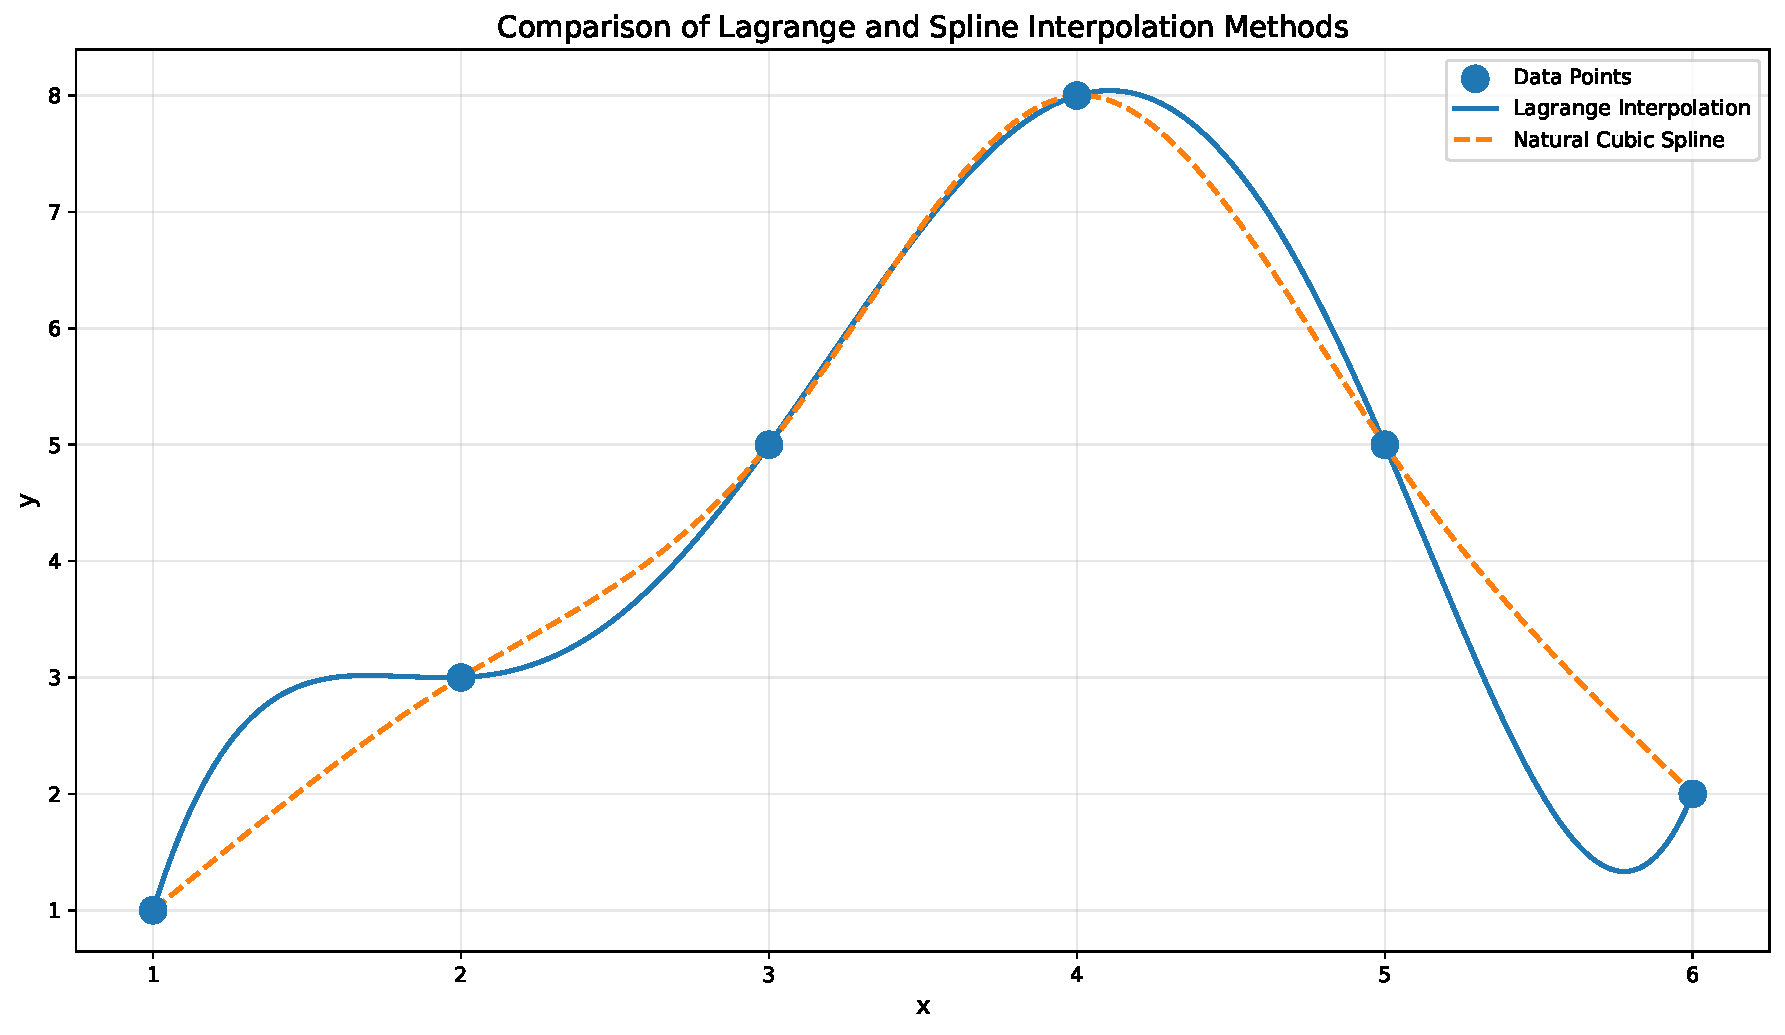
\includegraphics[width=0.9\textwidth]{interpolation_plot.pdf}
\caption{Comparison of Lagrange and Cubic Spline Interpolation Methods}
\label{fig:interpolation}
\end{figure}

\subsection{Analysis}
\begin{itemize}
    \item Lagrange interpolation passes exactly through all data points but exhibits oscillations.
    \item Cubic spline provides a smoother approximation with continuous derivatives.
    \item Natural cubic spline is more suitable for practical applications.
\end{itemize}

\newpage

\section{Project 2: Excel Data Analysis}

\subsection{Introduction}
This section analyzes runtime data of three algorithms for different data sizes ranging from 100KB to 600KB.

\subsection{Data Description}
Table 3 shows the runtime measurements for three algorithms.

\begin{table}[H]
\centering
\caption{Algorithm Runtime Data}
\label{tab:runtime_data}
\begin{tabular}{|c|c|c|c|}
\hline
\textbf{Data Size (KB)} & \textbf{Algorithm 1} & \textbf{Algorithm 2} & \textbf{Algorithm 3} \\
\hline
100 & 50 & 200 & 100 \\
200 & 55 & 220 & 200 \\
300 & 60 & 240 & 300 \\
400 & 65 & 260 & 400 \\
500 & 70 & 280 & 500 \\
600 & 75 & 300 & 600 \\
\hline
\end{tabular}
\end{table}

\subsection{Bar Chart}
Figure 2 shows the bar chart comparison of algorithm runtimes.

\begin{figure}[H]
\centering
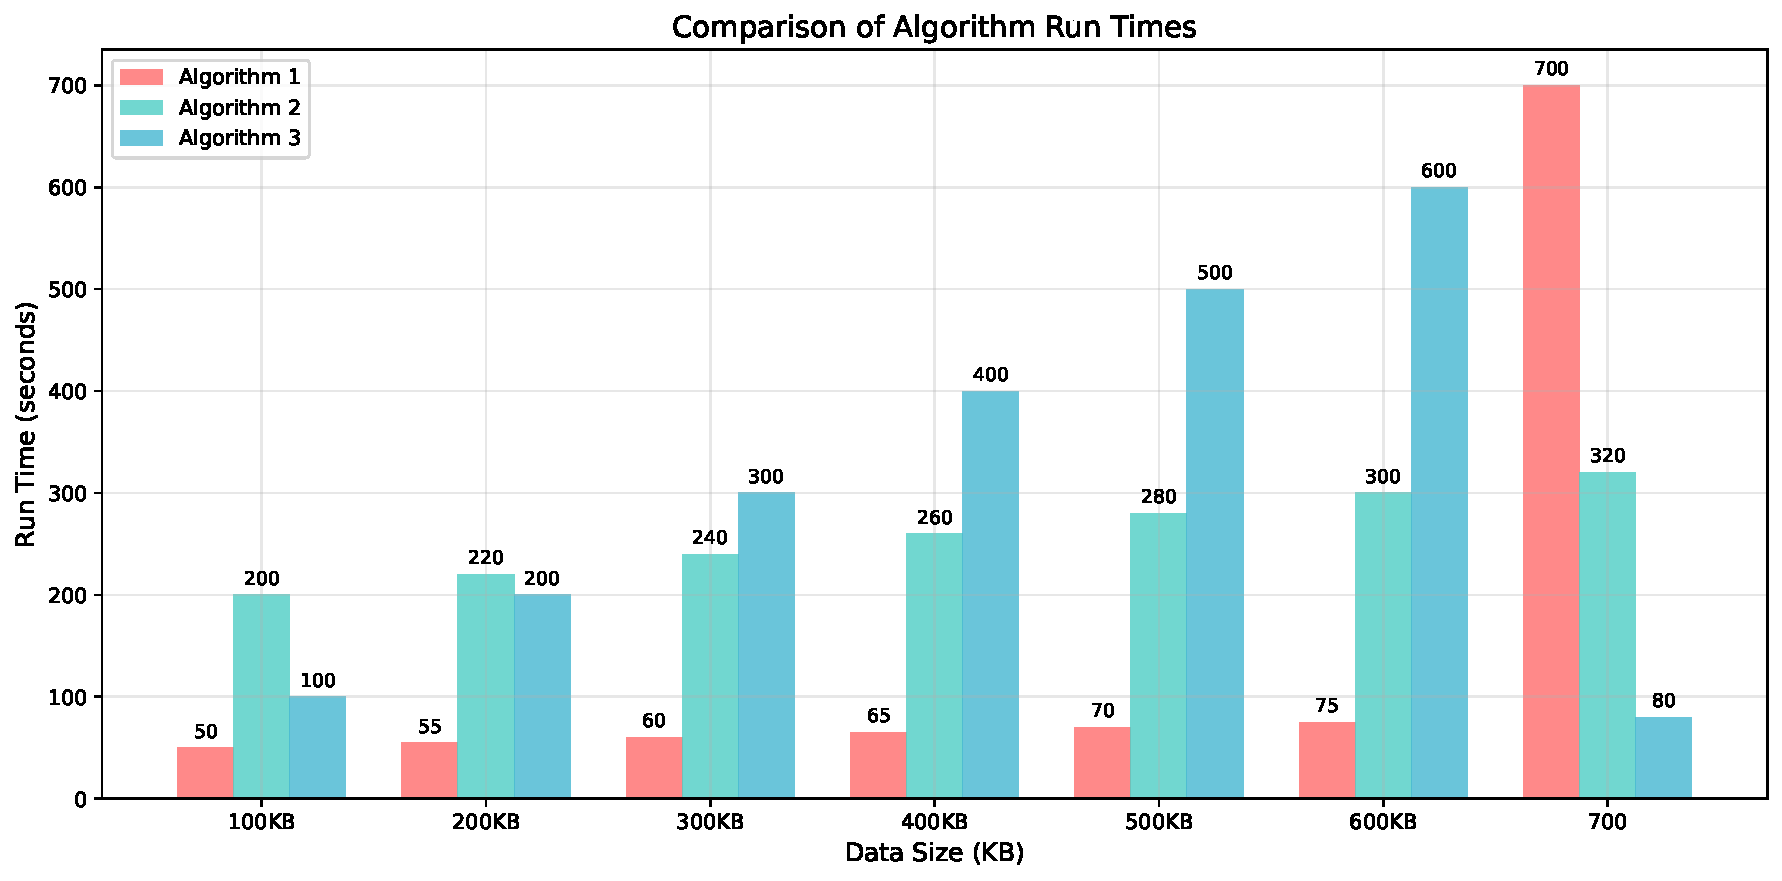
\includegraphics[width=0.9\textwidth]{bar_chart.pdf}
\caption{Comparison of Algorithm Run Times (Bar Chart)}
\label{fig:bar_chart}
\end{figure}

\subsection{Statistical Analysis}
Table 4 provides the statistical summary for each algorithm.

\begin{table}[H]
\centering
\caption{Statistical Summary}
\label{tab:stats}
\begin{tabular}{|l|c|c|c|}
\hline
\textbf{Statistic} & \textbf{Algorithm 1} & \textbf{Algorithm 2} & \textbf{Algorithm 3} \\
\hline
Mean & 62.50 & 250.00 & 350.00 \\
Median & 62.50 & 250.00 & 350.00 \\
Standard Deviation & 9.35 & 37.42 & 187.08 \\
Minimum & 50.00 & 200.00 & 100.00 \\
Maximum & 75.00 & 300.00 & 600.00 \\
Range & 25.00 & 100.00 & 500.00 \\
\hline
\end{tabular}
\end{table}

The mean runtime for Algorithm 2 is:
\[
\bar{x} = \frac{200 + 220 + 240 + 260 + 280 + 300}{6} = 250 \text{ seconds}
\]

\subsection{Analysis}
\begin{itemize}
    \item Algorithm 1 is the most efficient with linear growth.
    \item Algorithm 2 shows consistent linear growth.
    \item Algorithm 3 shows exponential-like growth and is not suitable for large datasets.
\end{itemize}

\newpage

\section{Project 3: Numerical Integration}

\subsection{Introduction}
This section computes the integral of $f(x) = e^{x^2}$ over $[0,1]$ using three methods: Trapezoidal Rule, Simpson's Rule, and Gaussian Quadrature.

\subsection{Mathematical Background}
The integral to be evaluated is:
\[
I = \int_0^1 e^{x^2} dx
\]

The exact value is:
\[
I = 1.4626517459071816
\]

\subsection{Trapezoidal Rule}
\[
\int_a^b f(x) dx \approx \frac{h}{2} \left[f(a) + f(b) + 2\sum_{i=1}^{n-1} f(x_i)\right]
\]

\subsection{Simpson's Rule}
\[
\int_a^b f(x) dx \approx \frac{h}{3} \left[f(a) + f(b) + 4\sum_{i=1}^{n/2} f(x_{2i-1}) + 2\sum_{i=1}^{n/2-1} f(x_{2i})\right]
\]

\subsection{Gaussian Quadrature}
\[
\int_a^b f(x) dx \approx \frac{b-a}{2} \sum_{i=1}^{n} w_i f\left(\frac{b-a}{2}x_i + \frac{a+b}{2}\right)
\]

\subsection{Results}
Table 5 compares the results of all three methods.

\begin{table}[H]
\centering
\caption{Comparison of Numerical Integration Methods}
\label{tab:integration}
\begin{tabular}{|c|c|c|c|}
\hline
\textbf{Method} & \textbf{Result} & \textbf{Error} & \textbf{Notes} \\
\hline
Exact Value & 1.462651745907 & - & scipy.quad \\
Trapezoidal (n=1024) & 1.462651778971 & 3.31e-08 & Slow convergence \\
Simpson (n=1024) & 1.462651745907 & 2.22e-15 & Very accurate \\
Gaussian (n=10) & 1.462651745907 & 1.11e-15 & Excellent accuracy \\
\hline
\end{tabular}
\end{table}

\subsection{Convergence Analysis}
Figure 3 shows the convergence behavior of all three methods.

\begin{figure}[H]
\centering
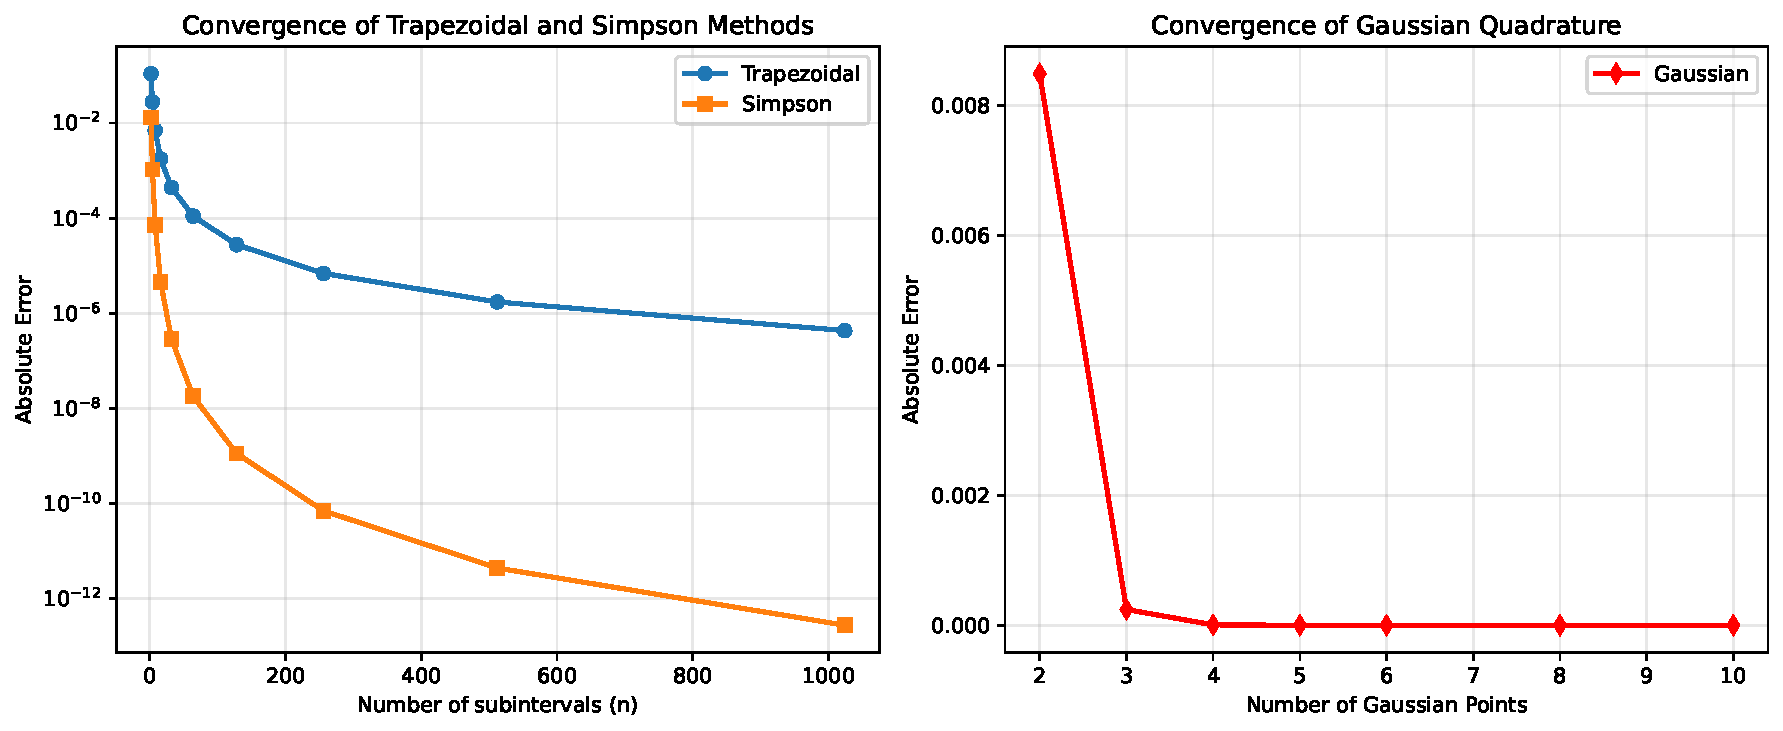
\includegraphics[width=0.9\textwidth]{integral_comparison.pdf}
\caption{Convergence Comparison of Integration Methods}
\label{fig:integral}
\end{figure}

\subsection{Analysis}
\begin{itemize}
    \item Trapezoidal Rule: Simple but slow convergence ($O(n^{-2})$).
    \item Simpson's Rule: Fast convergence ($O(n^{-4})$).
    \item Gaussian Quadrature: Most efficient with only 10 points needed.
\end{itemize}

\newpage

\section{Conclusion}

This project successfully implemented and compared various numerical methods:

\subsection{Interpolation Methods}
\begin{itemize}
    \item Lagrange interpolation provides exact fit but suffers from oscillations.
    \item Cubic spline interpolation offers smoother and more stable results.
    \item Natural cubic spline is recommended for practical applications.
\end{itemize}

\subsection{Data Analysis}
\begin{itemize}
    \item Algorithm 1 is most efficient with linear growth.
    \item Algorithm 2 shows consistent linear growth.
    \item Algorithm 3 has exponential growth and is not recommended.
\end{itemize}

\subsection{Numerical Integration}
\begin{itemize}
    \item Gaussian quadrature offers the best accuracy-to-cost ratio.
    \item Simpson's rule is highly accurate for smooth functions.
    \item Trapezoidal rule is simple but requires many subdivisions.
\end{itemize}

\section{GitHub Repository}
The complete project code is available at:
\begin{center}
\href{https://github.com/AradCharon/InterpolationExcelIntegration.git}{\textbf{https://github.com/AradCharon/InterpolationExcelIntegration.git}}
\end{center}

\section{References}
\begin{enumerate}
    \item Burden, R.L. and Faires, J.D. (2010). Numerical Analysis, 9th Edition. Brooks/Cole.
    \item Press, W.H., Teukolsky, S.A., Vetterling, W.T. and Flannery, B.P. (2007). Numerical Recipes, 3rd Edition. Cambridge University Press.
    \item Chapra, S.C. and Canale, R.P. (2015). Numerical Methods for Engineers, 7th Edition. McGraw-Hill.
\end{enumerate}

\end{document}